% !TEX TS-program = pdflatex
% !TEX encoding = UTF-8 Unicode

% This is a simple template for a LaTeX document using the "article" class.
% See "book", "report", "letter" for other types of document.

\documentclass[11pt]{article} % use larger type; default would be 10pt

\usepackage[utf8]{inputenc} % set input encoding (not needed with XeLaTeX)
\usepackage[QX]{fontenc}
\usepackage{lmodern}

%%% Examples of Article customizations
% These packages are optional, depending whether you want the features they provide.
% See the LaTeX Companion or other references for full information.

%%% PAGE DIMENSIONS
\usepackage{geometry} % to change the page dimensions
\geometry{a4paper} % or letterpaper (US) or a5paper or....
% \geometry{margin=2in} % for example, change the margins to 2 inches all round
% \geometry{landscape} % set up the page for landscape
%   read geometry.pdf for detailed page layout information

\usepackage{graphicx} % support the \includegraphics command and options
\usepackage{listings}
% \usepackage[parfill]{parskip} % Activate to begin paragraphs with an empty line rather than an indent

%%% PACKAGES
\usepackage{booktabs} % for much better looking tables
\usepackage{array} % for better arrays (eg matrices) in maths
\usepackage{paralist} % very flexible & customisable lists (eg. enumerate/itemize, etc.)
\usepackage{verbatim} % adds environment for commenting out blocks of text & for better verbatim
\usepackage{subfig} % make it possible to include more than one captioned figure/table in a single float
% These packages are all incorporated in the memoir class to one degree or another...

%%% HEADERS & FOOTERS
\usepackage{fancyhdr} % This should be set AFTER setting up the page geometry
\pagestyle{fancy} % options: empty , plain , fancy
\renewcommand{\headrulewidth}{0pt} % customise the layout...
\lhead{}\chead{}\rhead{}
\lfoot{}\cfoot{\thepage}\rfoot{}

%%% SECTION TITLE APPEARANCE
\usepackage{sectsty}
\allsectionsfont{\sffamily\mdseries\upshape} % (See the fntguide.pdf for font help)
% (This matches ConTeXt defaults)

%%% ToC (table of contents) APPEARANCE
\usepackage[nottoc,notlof,notlot]{tocbibind} % Put the bibliography in the ToC
\usepackage[titles,subfigure]{tocloft} % Alter the style of the Table of Contents
\renewcommand{\cftsecfont}{\rmfamily\mdseries\upshape}
\renewcommand{\cftsecpagefont}{\rmfamily\mdseries\upshape} % No bold!

%%% END Article customizations

%%% The "real" document content comes below...

\title{Metody obliczeniowe zadanie nr. 2}
\author{Mateusz Miotk \\ Sylwia Kaczmarczyk \\ Michał Kulesz}
\date{} % Activate to display a given date or no date (if empty),
         % otherwise the current date is printed 

\begin{document}
\maketitle

\section{Treść zadania}

$\textbf {Zadanie 2.7}$ Dla równania $f(x) = 0$, gdzie $f(x)=4-2x-\ln x$,wczytać $ a,b \in R$ takie, by $0<a<b$ oraz $f(a)\cdot f(b)<0$ Następnie dopóki "użytkownik się nie znudzi",wczytywać wartości $0<\varepsilon<1 $ i metodą połowienia na $[a,b]$ przybliżyć z dokładnością $\varepsilon$ rozwiązanie tego równania. Rozwiązanie to przybliżyć również metodą Newtona z $x_0=a$, przy czym $x_k$ będzie dobrym przybliżeniem, gdy $|x_k-x_{k-1}|\le \varepsilon$.Porównać ilość kroków wykonanych metodą połowienia i metodą Newtona. 

\section {Podstawa teoretyczna:}
\subsection{Metoda połowienia przedziału(bisekcji)}
Jeśli f jest funkcją ciągłą w przedziale $[a,b]$ i jeśli $f(a) \cdot f(b) < 0 $, a więc $f$ zmienia znak w $[a,b]$, to funkcja ta musi mieć zero w $(a,b)$. Jest to konsekwencja własności Darboux funkcji ciągłych. Metoda bisekcji korzysta z tej własności. Jeśli $f(a)f(b) < 0 $ to obliczamy $c=\frac{1}{2}(a+b)$ i sprawdzamy, czy $f(a)f(c) < 0$. Jeśli tak, to f ma zero w $[a,c]$; wtedy pod b podstawiamy c. W przeciwnym razie jest $f(c)f(b) < 0$; wtedy pod a podstawiamy c. Szukamy do momentu jeśli $sgn(a)=sgn(b)$ lub $f(c) \le \varepsilon$ 
\subsection{Metoda Newtona:}
Szukamy we funkcji f rozwiązania równania $f(x)=0$. Niech $r$ będzie takim zerem, a $x$ jego przybliżeniem. Jeśli $f''$ istnieje, to na mocy twierdzenia Taylora mamy: \\
$0=f(r)=f(x+h)=f(x)+hf'(x) + \theta(h^2)$
gdzie $h=r-x$.\\ Jeśli $h$ jest małe (czyli x jest bliskie r), to jest rozsądne pominięcie składnika $\theta(h^2)$ i rozwiązanie otrzymanego równania względem $h$. Daję to $h=-f(x)/f'(x)$.Jeśli $x$ jest przybliżeniem $r$, to $x-f(x)/f'(x)$ powinno być lepszym przybliżeniem tego zera. Dlatego z definicji metoda Newtona zaczyna od przybliżenia $x_0$ zera $r$ i polega na rekurencyjnym stosowaniu wzoru:\\
$x_{n+1}:=x_n - \frac{f(x_n)}{f'(x_n)}$ dla $(x\ge 0)$.
\section {Algorytm realizujący zadanie}
1.Program wczytuje wartości $a,b \in R$ gdzie $0<a<b$ oraz $f(a) \cdot f(b) < 0$ \\
2.Następnie wczytywana jest wartość $\varepsilon$ dopóki użytkownik się "nie znudzi", gdzie \\ $0<\varepsilon<1$. \\
3.W każdym wczytaniu $\varepsilon$ liczone jest rozwiązanie za pomocą algorytmu metody bisekcji oraz metody Newtona.
\subsection {Algorytm bisekcji}
Wykorzystany jest dany kod:
\begin{lstlisting}[firstnumber=100]
unsigned int M=0;
	double u,v,e,c,w;
	u=f(a);
	v=f(b);
	e=b-a;
	printf("METODA BISEKCJI: \n");
	while(sgn(u) != sgn(v)){
	M++;
	e/=2;
	c=a+e;
	w=f(c);
	printf("f(%lf)==%lf\n",c,w);
	if(fabs(w) < epsilon)
	break;
		if(sgn(w) != sgn(u)){
			b=c;
			v=w;
		}
		else{
			a=c;
			u=w;
		}
	}
\end{lstlisting}
Przybliżonym rozwiązaniem jest wartość c. \\ M oznacza ilość wykonanych kroków.\\\\\\\\\\
\subsection {Algorytm metody Newtona}
Wykorzystany jest dany kod:
\lstset{language=C}
\begin{lstlisting}[firstnumber=100]
unsigned M=0;
	double v=f(x_0);
	printf("f(%lf)==%lf\n",x_0,v);
	printf("METODA NEWTONA: \n");
	double x_1;
	if(fabs(v) < epsilon)
	return ;
		while(1){
		M++;
		x_1 = x_0 - v/f_bis(x_0);
		v=f(x_1);
		printf("f(%lf)==%lf\n",x_1,v);
		if(fabs(x_1-x_0) <= epsilon){
		break;
		}
		x_0=x_1;
	}
	printf("Przyblizone rozwiazanie: f(%lf)==%lf\n",x_1,v);
	printf("Ilosc krokow: %d\n",M);
\end{lstlisting}
 M oznacza ilość wykonanych kroków.
\subsection {Przykładowe rozwiązanie}
Wykres funkcji w przedziale $[0,10]$\\
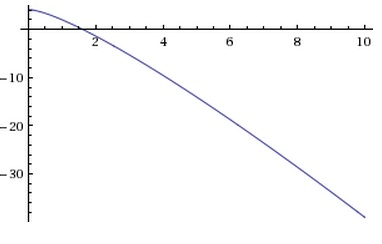
\includegraphics {Funkcja.jpg}\\
1.Dla danych:\\
$a=1$\\
$b=2$\\
$\varepsilon = 0.5$\\
Otrzymujemy :\\
METODA BISEKCJI:\\
f(1.500000)==0.594535\\
f(1.750000)==-0.059616\\
Przyblizone rozwiazanie: f(1.750000)==-0.059616\\
Ilosc krokow: 2\\
METODA NEWTONA:\\
f(1.666667)==0.155841\\
f(1.726606)==0.000632\\
Przyblizone rozwiazanie: f(1.726606)==0.000632\\
2.Dla danych:\\
$a,b$ - takie same jak wyżej \\
$\varepsilon = 0.01$\\
Otrzymujemy :\\
METODA BISEKCJI:\\
f(1.500000)==0.594535\\
f(1.750000)==-0.059616\\
f(1.625000)==0.264492\\
f(1.687500)==0.101752\\
f(1.718750)==0.020903\\
f(1.734375)==-0.019397\\
f(1.726562)==0.000743\\
Przyblizone rozwiazanie: f(1.726562)==0.000743\\
Ilosc krokow: 7\\
METODA NEWTONA:\\
f(1.666667)==0.155841\\
f(1.726606)==0.000632\\
f(1.726850)==0.000000\\
Przyblizone rozwiazanie: f(1.726850)==0.000000\\
Ilosc krokow: 3\\

\end{document}
